
% Strong background references addresses "what is already known" 
A climbing robot is a robot that moves on a vertical surfaces.
The idea was first suggested in a seminal work by Nishi et al.\cite{Nishi1986}
and has been revisited throughout for different application domains, 
including
%% The idea of developing climbing robots was expected for years but only in 1986, 
%% Nishi et al. presented in their seminal paper \cite{Nishi1986} 
%% the design of a robot that can walk on a vertical surface. During the last thirty years, many 
%% prototypes of climbing robots have been proposed for specific applications to replace 
%% humans in dangerous and difficult tasks, including inspection of
nuclear power 
plants \cite{Briones1994}, high-rise building cleaning \cite{Nansai2016}, bridges 
maintenance \cite{Wang2016}, search and rescue missions \cite{Eich2008}. 
However, % Mention a Gap in knowledge
there are still ways to climb walls not yet studied or reported \cite{bio_inspired2015}. 

% Introduction of the problem 
The research work done so far on climbing robots is reviewed and classified in 
\cite{Fang2022} and \cite{A.Hajeeretall2020}, respectively, according to the
adhesion technique \cite{longo2008} used to attach the robot to the
wall surface, and locomotion mechanism \cite{Chu2010}, utilized for
climbing.  The attachment and motion mechanisms are basically
considered as the main problems when designing climbing
robots. Additional requirements of equal importance come from the
application and include (R1) safety, and (R2) quickness in emergency
situations, (R3) carrying payloads, and (R4) avoiding
obstacles \cite{Schmidt2013}.

% Summarizing what's coming in the introduction
%In the coming two paragraphs, we give the reasons behind using a rope/wire 
%as an attachment method. After that, we suggest the jumping as moving technique.

\begin{figure}[t]
	\centering
	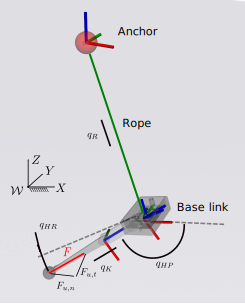
\includegraphics[width=0.7\columnwidth]{figs/3dmodel.pdf}
	\caption{\small Kinematic model of the CLIO robot with  standard definitions. The anchor frame is aligned with an inertial ($\mathcal{W}$) frame.}
	\label{fig:3dmodel}
\end{figure}


%% Solution for Attachment technique : USING A ROPE + main advantages   
Human climbers inspired the use of a rope mainly for safety measures (R1)
to support the weight of people during facade cleaning, firefighting and rescue missions
\cite{Nansai2016}.
In this paper, we combine the use of a rope with a leg, which can be retracted and extended
very quickly. This allows the robot to jump away from the mountain wall, while the rope
can be used to control its motion.

%Legged robots---as well as mobile robots---cannot walk on slopes with too high inclinations \cite{Abdalla12020} because limited friction results in slippage and falling.
%Instead, using a rope introduces an external force to compensate 
%for gravity (along the rope direction) and 
%allows the contact forces to satisfy the friction constraints (i.e., laying in 
%the middle of the friction cones) which ensures inherent safety (R1).
%
%% second advantage of using a rope : increase speed of movment 
Additionally, as shown by Wang et al. \cite{Wang2014} on dragline 
locomotion bio-inspired from spiders, the aid of rope can dramatically increase the locomotion speed (R2) 
by a winding and releasing mechanism, therefore being a preferable solution in applications
that require a prompt intervention such as Search $\&$ Rescue missions.  
%  
%% Third advantage 
Furthermore, ropes can support much heavier payloads (R3) than robots relying on sticky/adhesive approaches~\cite{Kim2008,Riskin2009}, because of the limited tangential component of the adhesive and leg actuation.
%the amount of payload that can be carried by sticky/adhesive based climbing 
%robots \cite{Kim2008,Riskin2009} is very limited due to the small tangential component of 
%the adhesive and leg actuation. Conversely, a feature of rope to be ideally 
%inextensible\footnote{The maximum payload will be limited by the maximum force deliverable 
%by the winding mechanism, e.g. a hoist, which can be extended using a gearbox.} \ADP{I don't see the connection between the rope being inextensible and the payload. The payload is large because gravity is compensated through the rope force instead of the contact force with the wall.}
%will allow the robot to carry a heavier payload (R3). 
%Difficulties due to the dynamics when using a rope
However, having the robot attached to a rope poses some challenges.
First, the robot is under-actuated because it cannot \textit{fully} control the position of its center of mass when 
not in contact with the wall. Second, the rope represents a \textit{unilateral} 
constraint (i.e. it can only pull and not push), which further complicates the already hybrid 
dynamics and the low control authority of this class of robots. 

% Providing a solution for second problem: locomotion technique, we can reach the target with jumps 
Finally, rather than slowly taking steps as walking mechanism, the robot can take one or multiple 
jumps like the rapid jumping Salto-1P shown in \cite{Haldane2017} to reach the desired locations, 
and overcoming obstacles.

%Difficulties in the jumping technique
To summarise, the key features of jumping with a rope that can be released, 
are related to the locomotion speed and the 
ability to address up to \textit{vertical} inclinations. 
However, the resulting motion of the 
robot (and so the possibility to reach the target) depends on: 1) the
impulse exerted on the wall at lift-off, 2) the winding/unwinding of the rope.
%
%Optimization for plannig 
Therefore, a planning strategy for this kind of motions should take 
into account both these factors, besides the under-actuation, 
the constraints posed by the rope, the actuator limits and the 
contact interaction (i.e. friction). 

Numerical optimisation is an attractive solution for these 
planning problems \cite{Nguyen2019,Ding2020}, since it allows to minimise some optimality criteria, 
while ensuring that the physical constraints are satisfied along the planning horizon. 
%
%Indeed, casting locomotion planning as an optimization problem
%allows one to represent high-level tasks and system dynamics using cost functions and 
%constraints. 
In this framework, different goals can also be pursued, such as minimising energy 
consumption or reaching the target in minimum time. 

\subsection{Proposed Approach and Contribution}
%
In this work, we present a novel robotic platform called CLIO  (CLImbing rObot) that is able to 
reach desired targets on a vertical (or slanted) wall with different frictional properties. 
We also propose a planning approach, based on numerical optimisation, 
to solve the jumping problem employing a simplified model of the dynamics.
To summarize, the contributions of the paper are:
\begin{itemize}
	\item a novel design of a jumping robot platform CLIO.
	\item an optimal control formulation to generate a jump 
	motion to reach a desired target while overcoming an obstacle, 
	based on a simplified model of the system, which results in reduced computation time.
	\item simulation experiments to validate the effectiveness of the proposed approach, 
	both using the simplified model and in a more realistic (Gazebo) simulation, considering the 
	full dynamics of the robot.
	\item (minor) a reachability analysis that  shows that 
	the region of achievable targets is limited by the friction coefficient at the lift-off location.
\end{itemize}
%
%\subsection{Outline}
%
The paper is organized as follows: Section \ref{sec:robot} gives an
overview of the robot platform and derives a simplified model of it.  
Section \ref{sec:motionP}  describes the optimization
problem to plan jump trajectories based on the simplified model. 
Simulations results are presented in Section \ref{sec:results}. 
Finally, we draw the conclusions in Section \ref{sec:conclusion}.
